\chapter{Problem Statement \& Feasibility Study}
A problem statement is a concise description of an issue to be addressed or a condition to be improved upon. It identifies the gap between the current (problem) state and desired (goal) state of a process or product.

A feasibility study is an analysis that considers all of a project's relevant factors—including economic, technical, legal, and scheduling considerations—to ascertain the likelihood of completing the project successfully.

\section{Customer's Problem}
We have many branch-offices across the country as well as outside the country. Our office staffs need frequent communication with one another regardless of the location. We need a customized, full-featured, Internet-based telephony system for cost-effective communication. We are currently using traditional telephony systems provided by the mobile-phone operators along with other Internet based solutions like WhatsApp. But they are not so flexible to meet our customizations. Moreover, cost is too high for international calling.

We need a mobile application that can be used to dial and receive calls with flexible functionality and low-cost for both national and international calls.

\section{Proposed Solution}
The proposed solution consists of a Private Branch Exchange (PBX) server accessible worldwide through the company's private network with the help of Internet. Users will have an android application installed in their mobile phones. The phone will remain connected to the PBX server using Internet connectivity.

\begin{figure}[H]
    \centering
    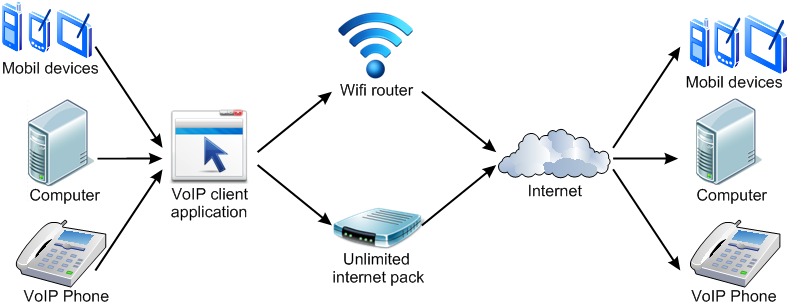
\includegraphics[width=.95\textwidth]{voip}
    \caption{VoIP Communication}
    \label{fig:voip}
\end{figure}

\section{Feasibility Study}
A feasibility study is an assessment of the practicality of a proposed project or system.

\subsection{Types of Feasibility Study}
The four types of feasibility include:
\begin{enumerate}
 \item \textbf{Technical}: Technology, hardware, and labor needed.
 \item \textbf{Financial}: The return on investment and the amount of funds needed to pay for the project, including the sources of capital, such as a financial institution or investors.
 \item \textbf{Market}: an analysis for the market for the product or service, the industry, competition, consumer demand, sales forecasts, and growth projections.
 \item \textbf{Organizational}: An outline of the business and the legal structure, as well as a management team analysis that includes a measurement of competency, such as the skills and experience needed.
\end{enumerate}

\subsection{Results of Our Study}

We did feasibility study on all the four types and found the project is worth doing. It is totally feasible and profitable to complete this project.

\begin{itemize}
 \item Technically feasible because all the tools, libraries and protocols require to complete this project are well-specified and easily obtainable. Asterisk can be used as a full-featured PBX server. PJSIP may be used as SIP User Agent Client (UAC).

 \item Financially feasible because it will reduce everyday call-costs to almost zero because of private PBX exchange. Moreover, its development cost and log-run maintenance cost is too low compared to the company's daily call costs.

 \item Organizational and Market feasibility are also OK because it does not need any special skills or experience required to use and operate the application for end-users.

\end{itemize}
